There are various ways in eCAD to draw entities. One can draw entities using draw menu, toolbar, shorcuts or commands. Each way is explained in detail as follows:
\subsection{Draw Menu}
We can draw the each entity using draw menu whether its point, line, circle, arc, ellipse, text or image. The way for each entity is described below.
\begin{figure}[h!]
\centering
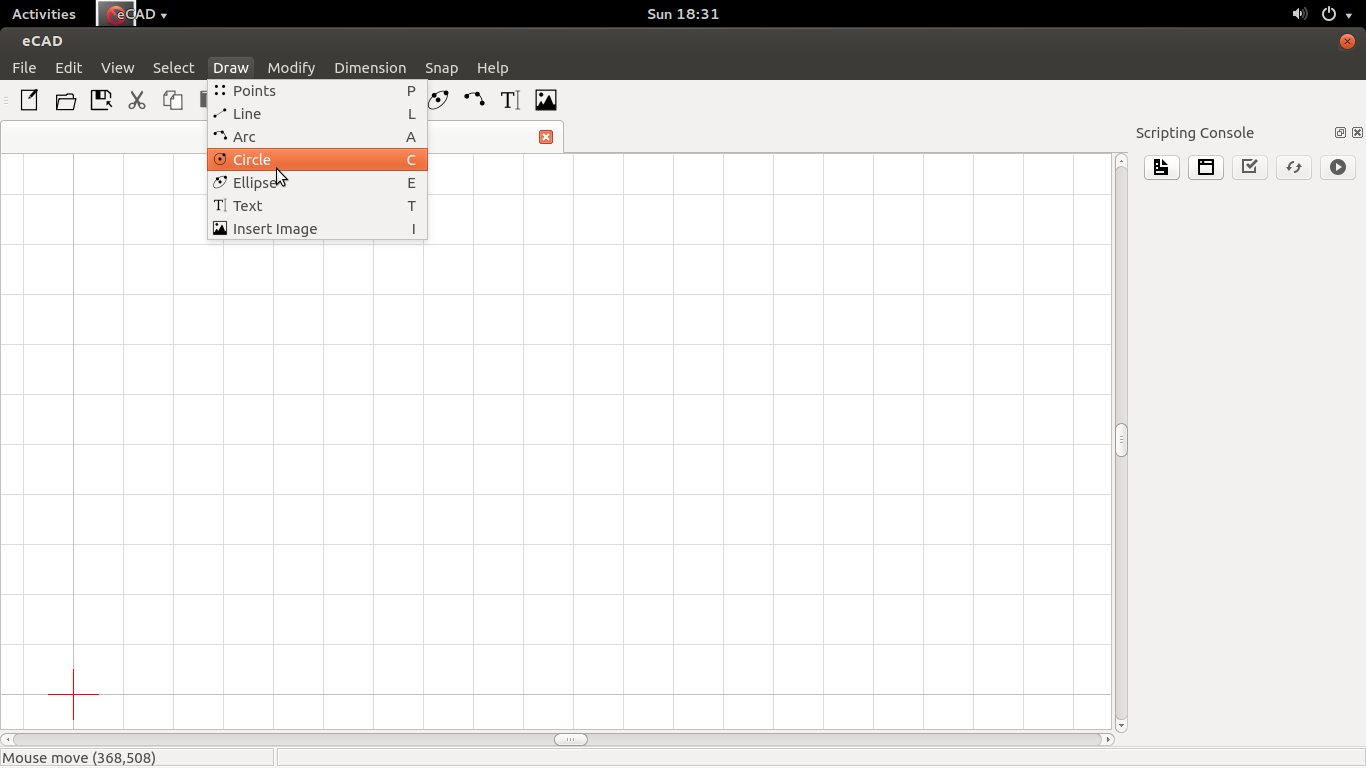
\includegraphics[width=0.7\textwidth]{images/drawmenu.png}\\
\end{figure}
\begin{enumerate}
\item \textbf{Point}
\begin{itemize}
\item Click on point in Draw menu
\item Then click anywhere on working space
\item This will create the point at that location.
\end{itemize}
\item \textbf{Line}
\begin{itemize}
\item Click on line in Draw menu
\item Then click first point on working space.
\item Set the second point of line.
\item This will create the line at two points.
\end{itemize}
\item \textbf{Arc}
\begin{itemize}
\item Click on arc in Draw menu
\item Click the start point of the arc
\item Then second click will create any point on the arc
\item Third click will create the end point of the arc
\item This will create our arc
\end{itemize}
\item \textbf{Circle}
\begin{itemize}
\item Click on circle in Draw menu
\item Then click on working area, this will create center point of arc
\item Second click will create any point on the circle and using first and second click radius of circle is calculated
\item This will create a circle.
\end{itemize}
\item \textbf{Ellipse}
\begin{itemize}
\item Click on point in Ellipse menu
\item Then click on graphics view this will create a center point of ellipse
\item After second click minor radius is calculated
\item After third click major radius is calculated
\item Finally ellipse is calculated
\end{itemize}
\item \textbf{Text}
\begin{itemize}
\item Click on text in Draw menu
\item Then click anywhere on working space
\item This will create a text box in which we can enter the text
\end{itemize}
\item \textbf{Image}
\begin{itemize}
\item Click on image in Draw menu
\item A dialog box will open, select an image to be inserted in it.
\item Then set the image where you want to set.
\end{itemize}
\end{enumerate}

\subsection{Toolbar}
Also we can draw the entities using the toolbar. The entities are in standard toolbar.
\begin{figure}[h!]
\centering
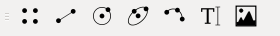
\includegraphics[width=0.7\textwidth]{images/entitytoolbar.png}\\
\end{figure}
\begin{enumerate}
\item \textbf{Point}
\begin{figure}[h!]
\centering
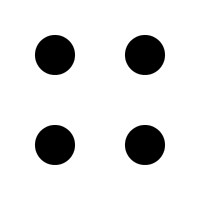
\includegraphics[width=0.05\textwidth]{images/point.jpg}\\
\end{figure}
\begin{itemize}
\item Click on above icon in toolbar
\item Then click anywhere on working space
\item This will create the point at that location.
\end{itemize}
\item \textbf{Line}
\begin{itemize}
\begin{figure}[h!]
\centering

\includegraphics[width=0.05\textwidth]{images/line.jpg}\\
\end{figure}
\item Click on above icon in toolbar
\item Then click first point on working space.
\item Set the second point of line.
\item This will create the line at two points.
\end{itemize}
\item \textbf{Arc}
\begin{figure}[h!]
\centering

\includegraphics[width=0.05\textwidth]{images/arc.jpg}\\
\end{figure}
\begin{itemize}
\item Click on above icon in toolbar
\item Click the start point of the arc
\item Then second click will create any point on the arc
\item Third click will create the end point of the arc
\item This will create our arc
\end{itemize}
\item \textbf{Circle}
\begin{figure}[h!]
\centering

\includegraphics[width=0.05\textwidth]{images/circle.jpg}\\
\end{figure}
\begin{itemize}
\item Click on above icon in toolbar
\item Then click on working area, this will create center point of arc
\item Second click will create any point on the circle and using first and second click radius of circle is calculated
\item This will create a circle.
\end{itemize}
\item \textbf{Ellipse}
\begin{figure}[h!]
\centering

\includegraphics[width=0.05\textwidth]{images/ellipse.jpg}\\
\end{figure}
\begin{itemize}
\item Click on above icon in toolbar
\item Then click on graphics view this will create a center point of ellipse
\item After second click minor radius is calculated
\item After third click major radius is calculated
\item Finally ellipse is calculated
\end{itemize}
\newpage
\item \textbf{Text}
\begin{figure}[h!]
\centering

\includegraphics[width=0.05\textwidth]{images/text.jpg}\\
\end{figure}
\begin{itemize}
\item Click on above icon in toolbar
\item Then click anywhere on working space
\item This will create a text box in which we can enter the text
\end{itemize}
\item \textbf{Image}
\begin{figure}[h!]
\centering

\includegraphics[width=0.05\textwidth]{images/image.jpg}\\
\end{figure}
\begin{itemize}
\item Click on above icon in toolbar
\item A dialog box will open, select an image to be inserted in it.
\item Then set the image where you want to set.
\end{itemize}
\end{enumerate}

\subsection{Shortcuts}
We can even create the entities using the shorcut keys.
\begin{enumerate}
\item \textbf{Point}
\begin{itemize}
\item Press P.
\item Then click anywhere on working space
\item This will create the point at that location.
\end{itemize}
\item \textbf{Line}
\begin{itemize}
\item Press L
\item Then click first point on working space.
\item Set the second point of line.
\item This will create the line at two points.
\end{itemize}
\item \textbf{Arc}
\begin{itemize}
\item Press A
\item Click the start point of the arc
\item Then second click will create any point on the arc
\item Third click will create the end point of the arc
\item This will create our arc
\end{itemize}
\item \textbf{Circle}
\begin{itemize}
\item Press C
\item Then click on working area, this will create center point of arc
\item Second click will create any point on the circle and using first and second click radius of circle is calculated
\item This will create a circle.
\end{itemize}
\item \textbf{Ellipse}
\begin{itemize}
\item Press E
\item Then click on graphics view this will create a center point of ellipse
\item After second click minor radius is calculated
\item After third click major radius is calculated
\item Finally ellipse is calculated
\end{itemize}
\item \textbf{Text}
\begin{itemize}
\item Press T
\item Then click anywhere on working space
\item This will create a text box in which we can enter the text
\end{itemize}
\item \textbf{Image}
\begin{itemize}
\item Press I
\item A dialog box will open, select an image to be inserted in it.
\item Then set the image where you want to set.
\end{itemize}
\end{enumerate}